\section{杰尼西亚的耳朵}
\markboth{6. 杰尼西亚的耳朵}{6. 杰尼西亚的耳朵}

\noindent
\begin{minipage}[t]{0.55\textwidth}
  \setlength{\parindent}{2em}
  据传说，在意大利西西里岛有一个山洞，很久以前，叙拉古的暴君杰尼西亚把他的一些囚犯关在这个山洞里。囚犯们多次密谋逃跑，但是每次的计划都被杰尼西亚发现了。起初，囚犯们怀疑自己的同伴中有内奸，他们彼此指责，互相猜疑，但是始终没有发现任何一个囚犯告密。后来渐渐觉察到囚禁他们的山洞形状古怪，洞壁把囚犯们的话都反射到狱卒的耳朵里去了，囚犯们诅咒这个山洞是“杰尼西亚的耳朵”。从图 6.1 可以看出，山洞的剖面近似于椭圆，犯人聚居的地方恰好在一个焦点附近，狱卒在另一个焦点偷听，无论囚犯们怎样压低嗓门，他们的声音照样被狱卒偷听得清清楚楚。
\end{minipage}
\hfill
\begin{minipage}[t]{0.42\textwidth}
  \centering
  \vspace{-2pt}
  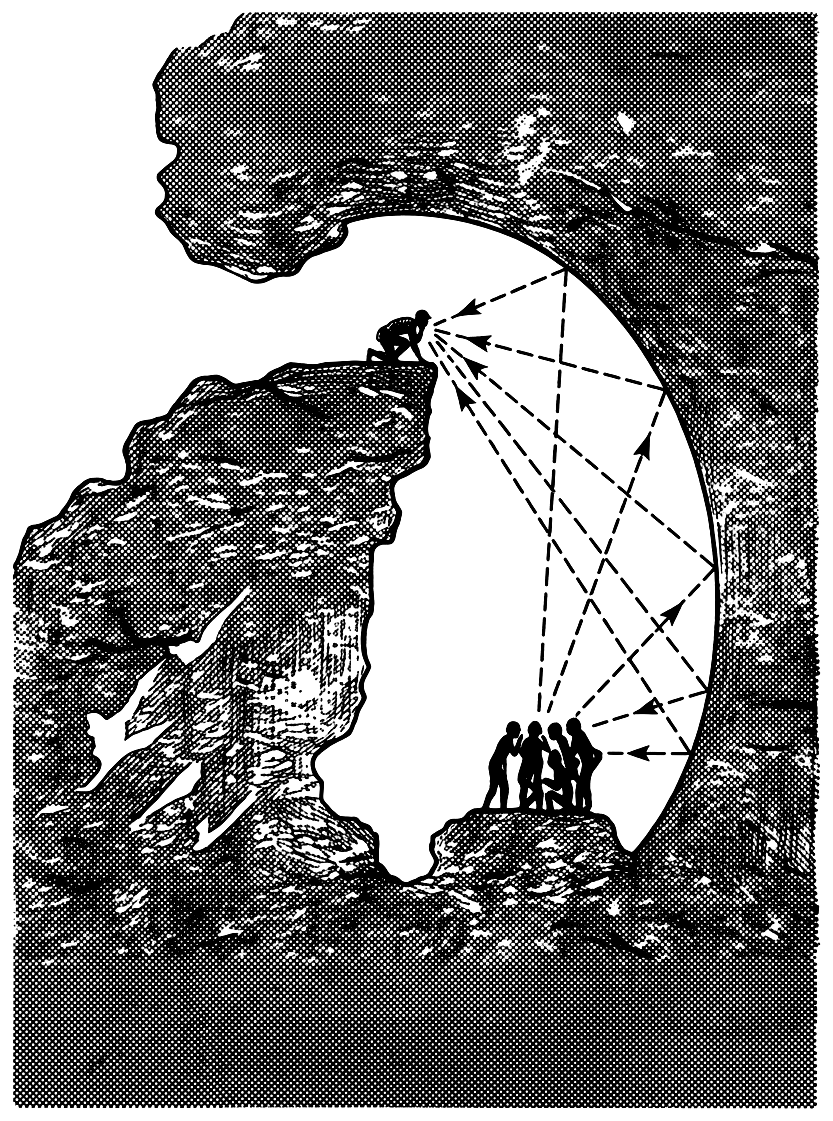
\includegraphics[width=\linewidth]{fig_006_1.png}
  \par\vspace{4pt}{\footnotesize 图\ 6.1}
\end{minipage}

这个传说表明，椭圆形的反射面不但能使从一个焦点发出的光线在另一个焦点会聚，而且能使从一个焦点发出的声音在另一个焦点聚焦。人们曾经发现一个古希腊音乐厅的墙壁正是椭圆形的，乐池位于一个焦点附近。在这个音乐厅里，乐队演奏的声音会在另一个焦点重新会聚起来。美国有一个教堂也有类似的设计，这种设计的出发点不得而知，其实声音的聚焦并不是好事，因为在另一焦点附近的听众固然连演奏或演讲者的细声慢语都能听见；但是在室内其它地方，音响效果却差得多。因而，现代在设计音乐厅、影剧院、大会堂等大型建筑物时，建筑设计人员都很注意设法避免声聚焦。
